\documentclass[12pt]{exam}
\usepackage{amsmath}
\usepackage{amssymb}
\usepackage{graphicx}
\usepackage{hyperref}
\usepackage{tikz}
\usepackage{amssymb}
\usepackage{mathpartir}
\usepackage{forest}
\usepackage[utf8]{inputenc}

\title{Chapter 1: Untyped Lambda Calculus}
\author{Type Theory and Formal Proof Reading Group}
\date{}

\begin{document}

\maketitle
\printanswers

\begin{questions}

	% 1.1
	\question Remove parenthesis, combine abstractions.

	Apply Notation 1.3.10 on the following $\lambda$-terms. So, remove parentheses and combine $\lambda$-abstractions:

	\begin{parts}
		\part
		$(\lambda x . (((x z) y) (x x)))$

		\begin{solution}

			Original term:
			\[
				(\lambda x . (((x z) y) (x x)))
			\]

			Applying Notation 1.3.10:
			\[
				(\lambda x . (((x z) y) (x x))) \implies \lambda x . (((x z) y) (x x)) \implies \lambda x . (((x z) y) (x x))
			\]
		\end{solution}

		\part
		$((\lambda x . (\lambda y . (\lambda z . (z ((x y) z))))) (\lambda u . u))$

		\begin{solution}

			Original term:
			\[
				((\lambda x . (\lambda y . (\lambda z . (z ((x y) z))))) (\lambda u . u))
			\]

			Applying Notation 1.3.10:
			% First, we substitute \( \lambda u . u \) for \( x \):
			\[
				((\lambda x . (\lambda y . (\lambda z . (z ((x y) z))))) (\lambda u . u)) \implies
				(\lambda x . (\lambda y . (\lambda z . (z ((x y) z))))) (\lambda u . u)
			\]

			Now simplify:\\
			\[
				\begin{array}{cl}
					  & (\lambda x . (\lambda y . (\lambda z . (z ((x y) z))))) (\lambda u . u) [x = \lambda u . u] \\
					= & (\lambda y . (\lambda z . (z (((\lambda u . u) y) z))))                                     \\
					= & (\lambda y . (\lambda z . (z (((\lambda u . u) y) z)))) [u = y]                             \\
					= & \lambda y . (\lambda z . (z (y z)))
				\end{array}
			\]
		\end{solution}
	\end{parts}



	% 1.2
	\question
	Which of the following are $\alpha$-equivalent to $\lambda x. x (\lambda x. x)$ ?

	\begin{parts}

		\part $\lambda y. y (\lambda x. x)$

		\begin{solution}
			$[x/y] \Rightarrow \lambda x. x (\lambda x. x)$

			So, yes.
		\end{solution}

		\part
		$\lambda y. y (\lambda x. y)$

		\begin{solution}
			No. Second abstraction's var uses outer abstraction's var.
		\end{solution}

		\part
		$\lambda y. y (\lambda y. x)$

		\begin{solution}
			No. $x$ is free.
		\end{solution}
	\end{parts}

	% 1.3
	\question
	Prove that $\lambda x. x (\lambda z. y) =_\alpha \lambda z. z (\lambda z. y)$.

	\begin{solution}

		\begin{tabular}{cll}
			  & $\lambda x. x (\lambda z. y)$ &                                      \\
			= & $\lambda z. z (\lambda z. y)$ & (Reason: $[z/x]$ $\alpha$-reduction) \\
		\end{tabular}

	\end{solution}

	% 1.4
	\question
	\begin{parts}
		\part
		Give U as its tree representation.

		\begin{solution}
			Based on the definition of diagrams as in Figure 1.1
			\begin{itemize}
				\item Application are joint points labelled 'a'.
				\item Abstraction are marked here with $\lambda$ (circled in book)
			\end{itemize}

			\begin{center}
				\begin{forest}
[a
    [$\lambda z$
      [a
        [z]
        [x]
      ]
      [z]
    ]
    [a
      [$\lambda y$
        [a
          [x]
          [y]
        ]
      ]
      [x]
    ]
]
				\end{forest}
			\end{center}
			beginbegin
		\end{solution}


		\part Generate free variables of $U$ (as in Examples 1.4.2).

		\begin{solution}
			Free variables can be found as:

			\begin{mathpar}
				\begin{array}{rcl}
					FV(x)            & = & x                \\
					FV(M N)          & = & FV(M) \cup FV(N) \\
					FV(\lambda x. M) & = & FV(M) \ {x}      \\
				\end{array}
			\end{mathpar}

			For given lambda term, the free variables are:

			\begin{mathpar}
				\begin{array}{cl}
					  & FV[(\lambda z. z x z)((\lambda y. x y) x)]       \\
					= & FV(\lambda z. z x z) \cup FV((\lambda y. x y) x) \\
					  & FV(\lambda z. z x z)                             \\
					\\
					= & FV((z x) z) \ {z}                                \\
					= & [FV(z x) \cup {z}] \ {z}                         \\
					= & [{z, x} \cup {z}] \ {z}                          \\
					= & {x}                                              \\
					\\
					  & FV((\lambda y. x y) x)                           \\
					= & FV(\lambda y. x y) \cup {x}                      \\
					= & [FV(x y) \ {y}] \cup {x}                         \\
					= & {x}
				\end{array}
			\end{mathpar}

			Therefore, the answer is: ${x} \cup {x}  = {x}$

		\end{solution}

		\part
		Find out which of the following $\lambda$-terms are $\alpha$-equivalent to $U$
		and give a motivation why; also check which of them satisfies the Barendregt
		convention:
		\begin{itemize}
			\item $(\lambda y. y x y)((\lambda z. x z) x)$
			\item $(\lambda x. x y x)((\lambda z. y z) y)$
			\item $(\lambda y. y x y)((\lambda y. x y) x)$
			\item $(\lambda v. (v x) v)((\lambda u. u v) x)$
		\end{itemize}

		\begin{solution}
			The last one is not $\alpha$-equiv to $U$ because of the second sub-term.
			All others are.

			Barendregt convention means to avoid using variables names that will
			cause shadowing and free variable capture.

			\begin{itemize}
				\item 1st one doesn't satisfy Barendregt conventions because of $(\lambda z. x z) x$
				\item Likewise 2nd one, because of $((\lambda z. y z) y)$
				\item Likewise 3rd one, because of $((\lambda y. x y) x)$
			\end{itemize}

			Last one:

			\begin{mathpar}
				\begin{array}{cl}
					  & (\lambda v. (v x) v) ((\lambda u. u v) x) \\
					= & (\lambda v. (v x) v) (x v)                \\
					= & ((x v) x) (x v)                           \\
				\end{array}
			\end{mathpar}

			So last one doesn't satisfy Barendregt convention either..
		\end{solution}

	\end{parts}

	% 1.5
	\question
	Perform the following substitutions: % 1.5
	\begin{parts}
		\part %(\lambda x. y(\lambda y. x y))[y := \lambda z. z x]
		$(\lambda x. \ y \ (\lambda y.\ x\ y))[y := \lambda z.\ z\ x]$

		\begin{solution}
			$(\lambda x.\ (\lambda z.\ z\ x)\ (\lambda y.\ x\ y))$
		\end{solution}

		\part
		$((x\ y\ z)[x\ :=\ y])[y\ :=\ z]$

		\begin{solution}

			\[
				\begin{array}{rl}
					  & ((x\ y\ z)[x\ :=\ y])[y\ :=\ z] \\
					= & ((x\ z\ z)[x\ :=\ y])           \\
					= & (y\ z\ z)                       \\
				\end{array}
			\]

		\end{solution}

		\part
		$((\lambda x.\ x\ y\ z)[x\ :=\ y])[y\ :=\ z]$

		\begin{solution}
			\[
				\begin{array}{rl}
					  & ((\lambda x.\ x\ y\ z)[x\ :=\ y])[y\ :=\ z] \\
					= & ((\lambda x.\ x\ z\ z)[x\ :=\ y])           \\
					= & (\lambda y.\ y\ z\ z)                       \\
				\end{array}
			\]
		\end{solution}

		\part
		$(\lambda y.\ y\ y\ x)[x\ :=\ y\ z]$

		\begin{solution}
			$(\lambda y.\ y\ y\ (y\ z))$
		\end{solution}

	\end{parts}

	% 1.6
	\question
		Show that the following propositions is not always true
		\[M[ x:=N, y:=L] = M[ x:=N]\,[ y:=L]\]
		
		\begin{solution}
		
		Counterexample:
		
		Let $M=x$, $N=y$, $L=z$ then
		\[M[ x:=N, y:=L] = x[ x:=y, y:=z] = y\]
		
		while 
		
		\[M[ x:=N]\,[ y:=L] = x[ x:=y]\,[y:=z] = y[y:=z] = z\]
		\end{solution}

	% 1.7
	\question
		Consider the term $U$ of exercise 1.4 
		\[U := (\lambda z. zxz) ((\lambda x. xy)x)\]
		\begin{solution}
		\begin{parts}
		\part
		 $U$ and $((\lambda x. xy)x)$
		\part
		All reduction paths of $U$:
		
		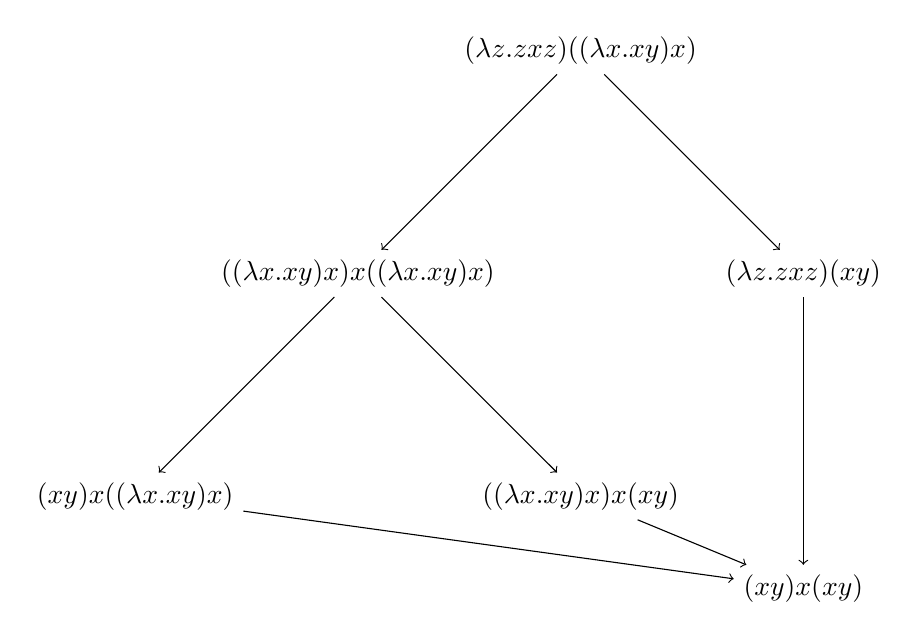
\begin{tikzpicture}[node distance =4 cm]
		\node[](A){$(\lambda z. zxz) ((\lambda x. xy)x)$};
		\node[](B)[below right of =A] {$(\lambda z. zxz)(xy)$};
		\node[](C)[below of=B]{$(xy)x(xy)$};
		\node[](D)[below left of = A]{$((\lambda x. xy)x) x ((\lambda x. xy)x)$};
		\node[](E) [below left of = D]{$(xy)x((\lambda x. xy)x)$};
		\node[](F) [below right of = D]{$((\lambda x. xy)x)x(xy)$};
		\draw[->]
		(A) edge (B)
		(B) edge (C)
		(A) edge (D)
		(D) edge (E)
		(D) edge (F)
		(E) edge (C)
		(F) edge (C);
		\end{tikzpicture}

		The $\beta$-normal form of $U$ is $(xy)x(xy)$.
		\end{parts}
		\end{solution}


	% 1.8
	\question
        Show that the terms ($\lambda$x . x x)y and ($\lambda$xy . y x)x x are not $\beta$-convertible.
        \begin{solution}
        
            ($\lambda$x . x x)y $\rightarrow_{\beta}$ (x x)[x := y] $\rightarrow_{\beta}$ y y $\rightarrow_{\beta}$ \\
            Can't be reduced further to a single term.\\
            ($\lambda$xy . y x)x x $\rightarrow_{\beta}$ ($\lambda$y . y x)[x := x] x $\rightarrow_{\beta}$ ($\lambda$y . y x) x  $\rightarrow_{\beta}$ (y x) [y := x] $\rightarrow_{\beta}$ x x\\
            Can't be reduced further to a single term.
            
        \end{solution}

	% 1.9
	\question
		Consider the following terms 
		\[K:=\lambda xy. x\]
		\[S:=\lambda xyz. xz(yz)\]
		
		\begin{solution}
		Redexes are underlined for clarity. Application of a mult-argument function is shown as one step. 
		\begin{parts}
		\part
		\[KPQ = \underline{(\lambda xy. x) PQ} \twoheadrightarrow_\beta P
		\]
		and 
		\[\underline{SPQR}= \underline{(\lambda xyz. xz(yz)) PQR}\twoheadrightarrow_\beta PRQR
		\]
		
		\part
		\[\underline{SKK} \twoheadrightarrow_\beta \lambda z. \underline{Kz(Kz)}\twoheadrightarrow_\beta \lambda z. z\]
		
		\part
		\begin{align*}
		BUVW &= \underline{S(KS)KU}VW \\
		&\twoheadrightarrow_\beta \underline{(KS)U}(KU)VW \\
		&\twoheadrightarrow_\beta \underline{S(KU)VW }\\
		&\twoheadrightarrow_\beta \underline{(KU)W}(VW) \\
		&\twoheadrightarrow_\beta U(VW)
		\end{align*}
		
		\part
		\[
		\underline{SKKK} \twoheadrightarrow_\beta \underline{KK(KK)} \twoheadrightarrow_\beta K
		\]
		and 
		\[
		\underline{SSSK}K \twoheadrightarrow_\beta \underline{SK(SK)K} \twoheadrightarrow_\beta \underline{KK((SK)K)} \twoheadrightarrow_\beta K
		\]
		\end{parts}
		\end{solution}

	% 1.10
	\question Given the following
		\[zero:=\lambda fx. x\]
		\[one:=\lambda fx. f x\]
		\[two:=\lambda fx. f (f x)\]
		\[add:=\lambda mnfx. m f (n f x)\]
		\[mult:=\lambda mnfx. m (n f) x\]
		\begin{solution}
		\begin{parts}
		\part
		\[\underline{\mathit{add} \mathit{one} \mathit{one}} \twoheadrightarrow_\beta \lambda fx. \underline{\mathit{one} f (\mathit{one} f x)} \twoheadrightarrow_\beta \lambda fx. f \underline{(\mathit{one} f x)} \twoheadrightarrow_\beta \lambda fx. f (f x) = \mathit{two} \]
		
		\part
		From (a) we know the $\beta$-normal form of $\mathit{add} \mathit{one} \mathit{one}$ is $\mathit{two}$. 
		We also have
		\[\underline{\mathit{mult} \mathit{one} \mathit{zero}} \twoheadrightarrow_\beta \lambda fx. \underline{\mathit{one} (\mathit{zero} f) x} \twoheadrightarrow_\beta \lambda fx. \underline{(\mathit{zero} f) x}  \twoheadrightarrow_\beta \lambda fx. x = zero\]
		so the $\beta$-normal form of $\mathit{mult} \mathit{one} \mathit{zero}$ is $\mathit{zero}$, and $\mathit{two} \neq \mathit{zero}$
		\end{parts}
		\end{solution}

	% 1.11
	\question

	% 1.12
	\question

	% 1.13
	\question

	% 1.14
	\question

	% 1.15
	\question

	% 1.16
	\question

	% 1.17
	\question

	% 1.18
	\question

	% 1.19
	\question

	% 1.20
	\question

\end{questions}

\end{document}
